\section{Einleitung}
\label{sec:Einleitung}
Zu den anderen orthopädischen Krankheitsbildern gehört auch der Ellenbogen. Es liegt also ein Befund des linken Ellenbogens (Epicondylitis ulnaris) und das soll im weiteren Verlauf näher untersucht werden.

\section{Patientenvorstellung}
\label{sec:Vorstellung}
Seit November 2015 hat eine Patientin Beschwerden beim linken Ellenbogen. Für eine Linderung der Symptome hat sie eine Reihe von konservativen Therapiemaßnahmen durchgeführt. Dazu gehört vor allem Ruhigstellung, Kühlung und Salbentherapie. Diese konservativen Therapiemaßnahmen haben leider nicht geholfen und die Patientin muss in die Strahlentherapie um am linken Ellenbogen bestrahlt zu werden. Hierbei wurden ihr die möglichen Wirkungen und Nebenwirkungen der Strahlentherapie durch den Arzt aufgeklärt. Diese wurden erfolgreich zur Kenntnis genommen. Zur weiteren Diagnosen gehören eine Schilddrüsenunterfunktion und Polyarthrose. Sie ist $\SI{168}{\centi\meter}$ groß, wiegt $\SI{78}{\kilo\gram}$ und die medialen Druckschmerzen befindet sich am linken Ellenbogen. Durch diese Schmerzen wird ihre Bewegung auch beeinträchtigt. Für die Bestrahlungsplanung gehört eine Gesamtdosis von $\SI{30}{\gray}$, welche in Fraktionen von $\SI{0,5}{\gray}$ in insgesamt 6 Bestrahlungen appliziert werden soll. Insgesamt sollen 3 Bestrahlungen pro Woche stattfinden. Das ist hilfreich, denn der Körper muss Zeit genug haben, auf die Behandlung zu reagieren. Falls es nach 8-10 Wochen keine Besserung ergibt, muss die Strahlentherapie wiederholt werden.

\section{Bestrahlungsplanung}
\label{sec:Bestrahlung}
Das PTV ist in den CT-Daten bereits eingezeichnet und als nächstes wurde die Kontur des Ellenbogens als Body-Struktur eingezeichnet. Andere Gegenstände, wie z.B. Lagerungshilfe oder Patientenliege, werden als Struktur eingezeichnet, weil sich diese auch im Strahlengang befinden. Dosiert wird hier auf den ICRU Referenzpunkt und das Ziel der Bestrahlungsplanung ist, dass das Planungszielvolumen durch die $\SI{95}{\percent}$ Isodosenlinie umschlossen wird. Das Dosismaximum soll bei $\SI{106}{\percent}$ liegen. Für die Bestrahlungsplanung wurden zwei Felder mit einer Gewichtung von 0.5 erzeugt. Die beiden Felder sind gleich groß und haben eine Größe von $\SI{12}{\centi\meter}$ x $\SI{16,5}{\centi\meter}$. Beim ersten Feld gibt es eine Gantry-Rotation von $0^\circ$ und beim zweiten eine Gantry-Rotation von $180^\circ$. Der Bestrahlungsplan wird auf "$\SI{100}{\percent}$ target mean" normiert. Für eine Schonung des umliegenden Gewebes werden MLCs verwendet, die an die Struktur angepasst werden können. Das ist in der Abbildung  zu sehen. 

\begin{figure}[htpb]
	\centering
	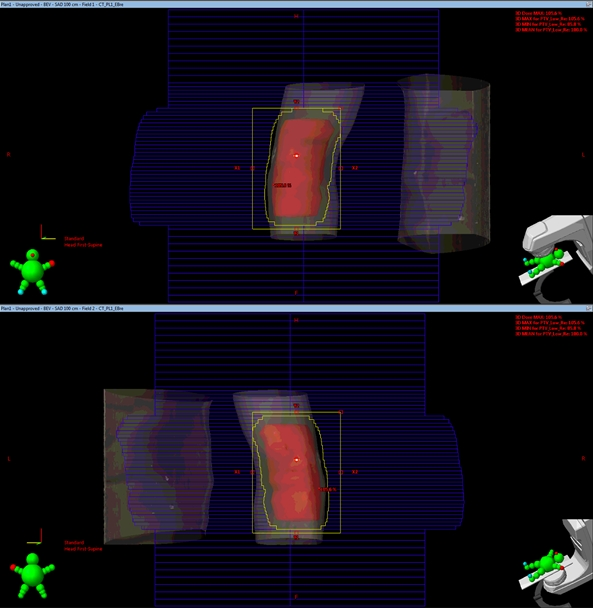
\includegraphics[width=0.7\linewidth]{../Bilder/kombi}
	\caption{Zu sehen ist die Darstellung der Lamellen beim MLC. Beim oberen Bild handelt es sich um das Feld bei $0^\circ$ und beim unteren Bild handelt es sich um das Feld bei $180^\circ$.}
	\label{fig:kombi}
\end{figure}


\section{Auswertung und Diskussion}
\label{sec:AuswertundDiskussion}
In den Abbildungen \ref{fig:ellenbogenx}, \ref{fig:ellenbogeny} und \ref{fig:ellenbogenz} sind die Dosisverteilungen des Ellenbogens in der Transversal-, Sagittal- und Frontalansicht zu sehen. In den Abbildungen ist zu erkennen, dass die $\SI{95}{\percent}$ Isodosenlinie zumindest in der Frontal- als auch der Transversalansicht nicht ganz das rote eingezeichnete PTV umschließt. Bei der Sagittalansicht wird das dennoch eingehalten. 
Damit das PTV mit der $\SI{95}{\percent}$ Isodosenlinie umgeschlossen werden kann, wäre es möglich für eine bessere Dosisverteilung zumindest die MLCs etwas genauerer einzustellen, die Felder zu vergrößern oder weitere Felder zu erzeugen.

\begin{figure}[htpb]
	\centering
	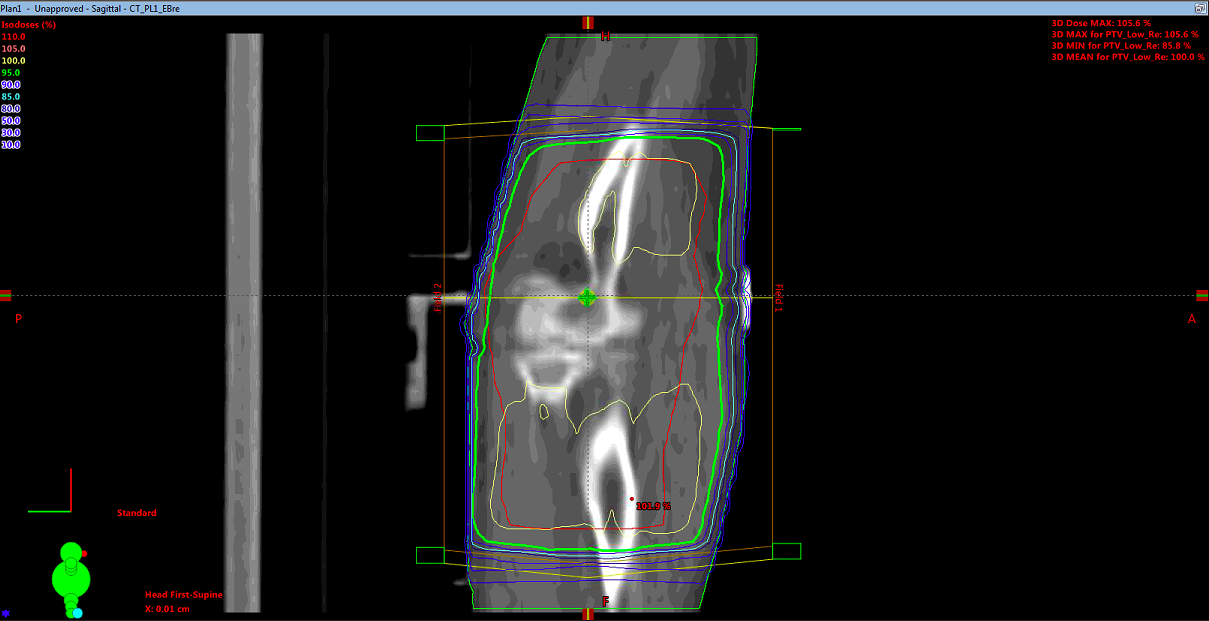
\includegraphics[width=0.7\linewidth]{../Bilder/EllenbogenX}
	\caption{Darstellung der Dosisverteilung in der Frontalansicht des Ellenbogens.}
	\label{fig:ellenbogenx}
\end{figure}

\begin{figure}[htpb]
	\centering
	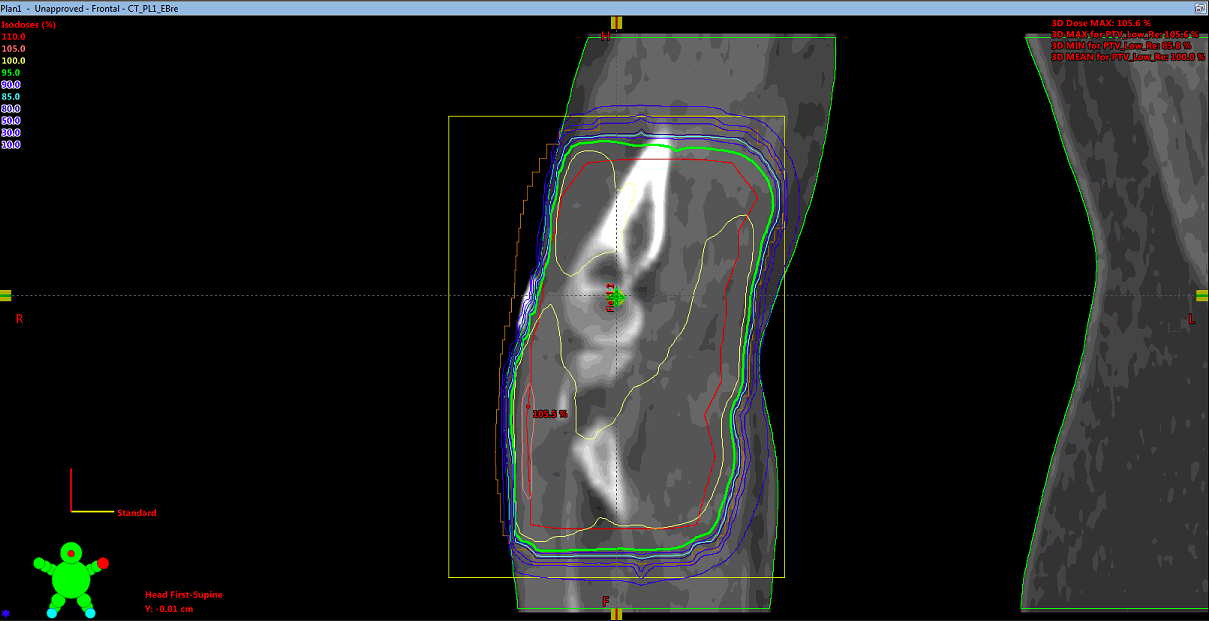
\includegraphics[width=0.7\linewidth]{../Bilder/EllenbogenY}
	\caption{Darstellung der Dosisverteilung in der Sagittalansicht des Ellenbogens.}
	\label{fig:ellenbogeny}
\end{figure}

\begin{figure}[htpb]
	\centering
	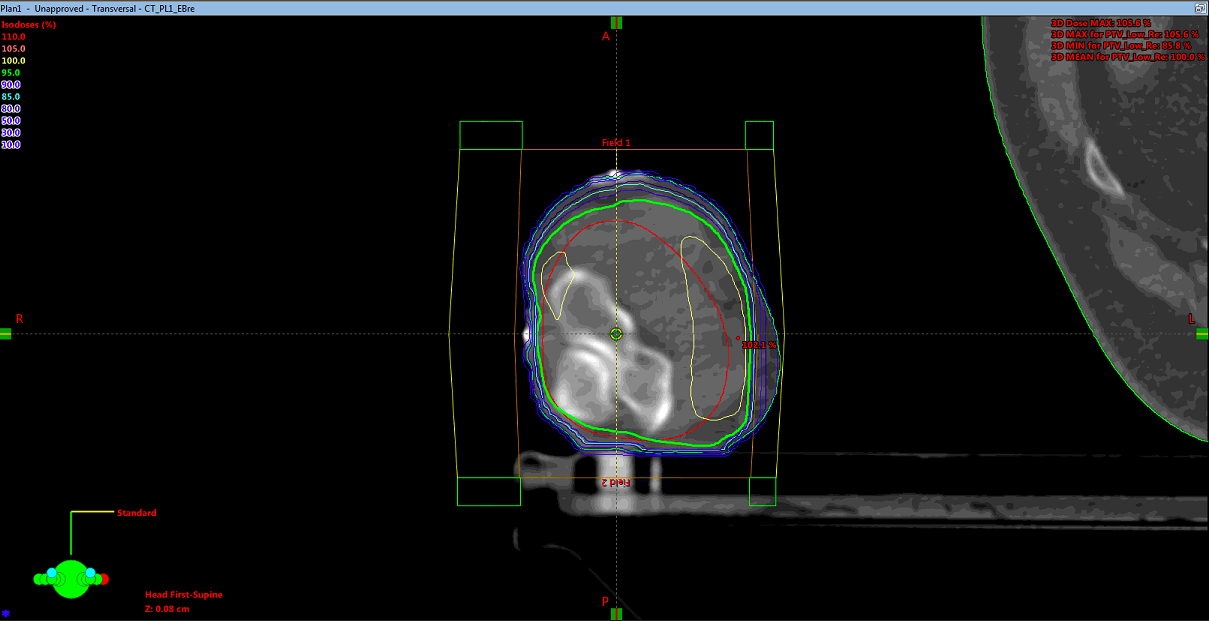
\includegraphics[width=0.7\linewidth]{../Bilder/EllenbogenZ}
	\caption{Darstellung der Dosisverteilung in der Transversalansicht des Ellenbogens.}
	\label{fig:ellenbogenz}
\end{figure}

Für eine bessere Beurteilung wurde ein Dosis-Volumen-Histogramm in der Abbildung \ref{fig:dvhellenbogeneinzel} erstellt. Die maximale Dosis, die bis zu $\SI{106}{\percent}$ im PTV betragen soll, liegt hier bei $\SI{105,6}{\percent}$ und wurde dementsprechend eingehalten. Das umliegende Gewebe wird auch geschont. Die minimale Dosis, die im PTV deponiert wird, liegt bei $\SI{85,8}{\percent}$. 
Das bedeutet, dass das gesamte PTV mit der $\SI{95}{\percent}$ - Isodosenlinie nicht bestrahlt wurde. Eine Möglichkeit dafür, wäre auf die Frontal- und Transversalansicht zurückzuführen, da dort das PTV nicht ganz umschlossen wurde. Allerdings ist das nur ein geringer Teil, der in der DVH nicht zu sehen ist. Wenn $\SI{100}{\percent}$ des PTVs mit der $\SI{95}{\percent}$ Isodosenlinie umschlossen wären, dann wäre auch die minimale Dosis $\SI{95}{\percent}$. Was noch erkennbar ist, ist dass $\SI{99,85}{\percent}$ des PTVs noch $\SI{95}{\percent}$ Dosis bekommt.

\begin{figure}[htpb]
	\centering
	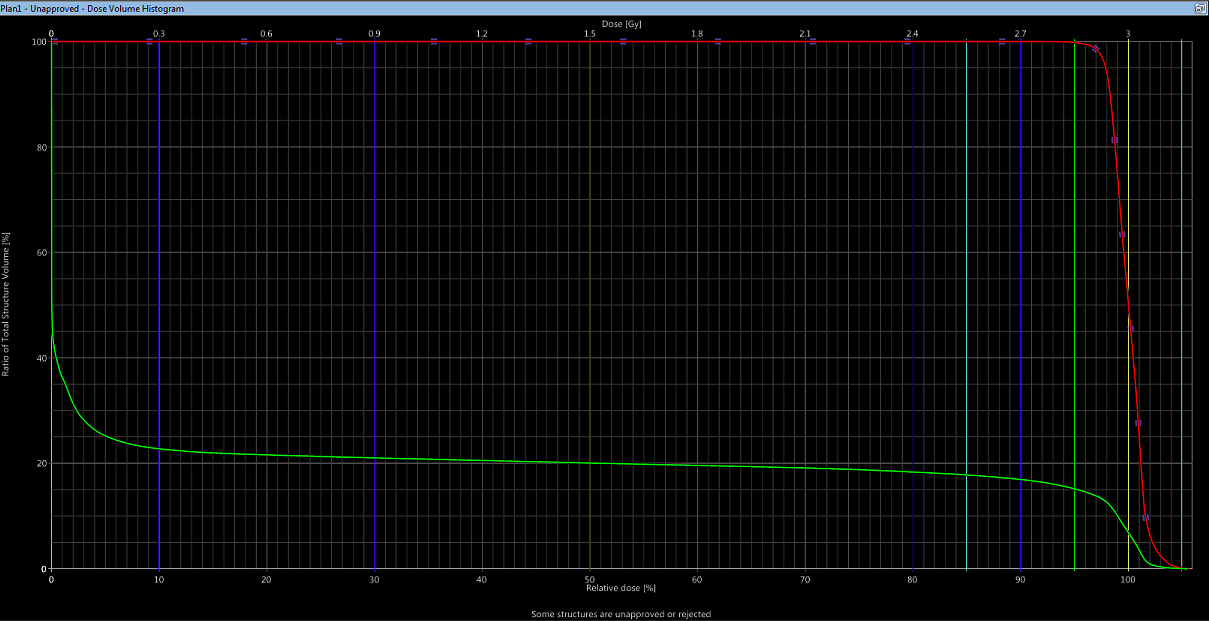
\includegraphics[width=0.7\linewidth]{../Bilder/DVH_EllenbogenEinzel}
	\caption{Zu sehen ist das Dosis-Volumen-Histogramm des Ellenbogens. In roter Farbe dargestellt ist das PTV und in grüner Farbe ist das Ellenbogen. Außerdem sind noch die einzelnen Isodosenlinie eingezeichnet.}
	\label{fig:dvhellenbogeneinzel}
\end{figure}

